\documentclass[18pt]{article}
\usepackage[a4paper, total={6.5in, 8.5in}]{geometry}
\usepackage[linesnumbered,ruled,vlined]{algorithm2e}
\usepackage{caption}
\usepackage{subcaption}
\usepackage{amsmath}
\usepackage{tikz}
\usepackage{hyperref}
\usepackage{rotating}
\usepackage{ragged2e}
\usepackage{float}
\usepackage[backend=biber,style=numeric]{biblatex}
\addbibresource{ref.bib} % Add your .bib file here
% Replace 'ref' with your .bib filename (without .bib extension)

\usetikzlibrary{arrows.meta}  % For arrow styles
\usetikzlibrary{shapes.geometric, positioning} % For shapes like rectangles, circles, and positioning nodes
\usepackage{xcolor}           % For colored boxes and text
\usetikzlibrary{positioning}

% Define colors
\definecolor{myblue}{RGB}{0, 102, 204}
\definecolor{mygreen}{RGB}{0, 153, 0}


% Declare lengths

\setlength{\parskip}{1em}

\newlength{\leafnodewidth} 
\newlength{\leafnodeheightone} 
\newlength{\leafnodeheighttwo}
\newlength{\leafnodetextstart}
\newlength{\leafnodetextend}

\newlength{\internalnoderadius}

\newlength{\leveldistance}

% Set length values

\setlength{\leafnodewidth}{6mm}
\setlength{\leafnodeheightone}{3mm}
\setlength{\leafnodeheighttwo}{9mm} 

\setlength{\leafnodetextstart}{11mm}
\setlength{\leafnodetextend}{15mm}

\setlength{\internalnoderadius}{3.5mm}

\setlength{\leveldistance}{14mm}

% Declare colors
\definecolor{leafcolorone}{RGB}{255,0,0} % red
\definecolor{leafcolortwo}{RGB}{0,0,255} % blue
\definecolor{internalnodecolor}{RGB}{0,255,0} % green
\definecolor{highlightededgecolor}{RGB}{139,1,102} %dark magenta
\definecolor{codecolorone}{RGB}{139,1,102} %dark magenta
\definecolor{codecolortwo}{RGB}{45, 141, 38} % dark green
\definecolor{dimcolor}{RGB}{217, 217, 217}


% Define the \leafnode command
\newcommand{\leafnode}[6]{
	\begin{tikzpicture}
		\filldraw[color=#1!90, fill=#1!3, thick, font=\tiny] (0,0) rectangle (\leafnodewidth, -\leafnodeheightone) node[midway, text=#3] {#4};
		\filldraw[color=#2!90, fill=#2!3, thick, font=\small] (0,-\leafnodeheightone) rectangle (\leafnodewidth, -\leafnodeheighttwo) node[midway, text=#3] {#5};
		
		% the following portion is only for showing after demonstration
		
		%\filldraw[color=white!100, fill=white!100, thick, font=\scriptsize] (0,-\leafnodetextstart) rectangle (\leafnodewidth, -\leafnodetextend) node[midway, text=#3] {#6};
		
	\end{tikzpicture}
}


% Define the \leafnode command
\newcommand{\labelledleafnode}[6]{
	\begin{tikzpicture}
		\filldraw[color=#1!90, fill=#1!3, thick, font=\tiny] (0,0) rectangle (\leafnodewidth, -\leafnodeheightone) node[midway, text=#3] {#4};
		\filldraw[color=#2!90, fill=#2!3, thick, font=\small] (0,-\leafnodeheightone) rectangle (\leafnodewidth, -\leafnodeheighttwo) node[midway, text=#3] {#5};
		
		\filldraw[color=violet!100, fill=white!100, thick, font=\scriptsize] (0,-\leafnodetextstart) rectangle (\leafnodewidth, -\leafnodetextend) node[midway, text=#3] {#6};
		
	\end{tikzpicture}
}

% Define the \internalnode command with a color argument
\newcommand{\internalnode}[3]{
	\begin{tikzpicture}
		\filldraw[color=#1!90, fill=#1!5, thick, font=\scriptsize] (0,0) circle (\internalnoderadius) node[midway, text=#2] {#3};
	\end{tikzpicture}
}


% Minimum Indicator
\newcommand{\mindicator}[0]{
	
	\vspace{0.5mm}
	
	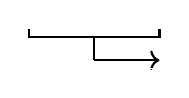
\begin{tikzpicture}
		
		\draw[black, thick] (0,0.1) -- (0,0) -- (1.66,0) -- (1.66,0.1);
		\draw[black, thick] (0.83,0) -- (0.83,-0.3);
		\draw[black, thick, ->] (0.83,-0.3) -- (1.66,-0.3);
		% Adding a dummy line for better positioning of the text
		\draw[white] (0,-0.4) -- (1.66,-0.4);
		
		
	\end{tikzpicture}
	\footnotesize{Minimum-weighted two nodes}
	
}






\title{CSE 200 \\
	Technical Writing and Presentation \\
	
	\vspace{5mm}
	
	\begin{figure}[h]
		\centering
		\includegraphics[width=0.3\textwidth]{images/buet.png}
		\label{fig:enter-label}
	\end{figure}
	
	\textbf{EasyJailbreak: A Unified Framework for Jailbreaking Large Language
	Models}}
\author{
	\textbf{Report written by:} \\
	2105032 - Nawriz Ahmed Turjo\\
	2105047 - Himadri Gobinda Biswas\\
	2105048 - Shams Hossain Simanto \\ \\
	\textbf{Section:} A2\\
	\textbf{Group:} 1\\ \\
	Department of Computer Science and Engineering\\
	Bangladesh University of Engineering and Technology\\
}
\date{December 18, 2024}




\tikzstyle{level 1} = [sibling distance=38mm]
\tikzstyle{level 2} = [sibling distance=30mm]
\tikzstyle{level 3} = [sibling distance=19mm]
\tikzstyle{visible_edge} = [->, draw, leafcolortwo, thick]
\tikzstyle{edge from parent} = [draw, teal, thick]
\tikzstyle{emph} = [edge from parent/.style={->,highlightededgecolor,draw,ultra thick}]
\tikzstyle{norm} = [edge from parent/.style={draw, teal, thin}]
\tikzstyle{noedge} = [edge from parent/.style={draw, white, thin}]

\tikzstyle{every node} = [inner sep=0]




\begin{document}
	\maketitle
	%\pagenumbering{roman}
	\pagebreak
	
	\setlength{\parskip}{0.5em}
	
	\tableofcontents
	
	\setlength{\parskip}{1em}
	%\setcounter{tocdepth}{2}
	\newpage
	
	\listoffigures
	\newpage
	
	\listoftables
	\newpage
	
	\newpage
	
	\section*{Abstract}	
	
	Jailbreak attacks are crucial for identifying and mitigating the security vulnerabilities of Large Language Models (LLMs). They are designed to bypass safeguards and elicit prohibited outputs.  
        However, due to significant differences among various jailbreak methods, there is no standard implementation framework available for the community, which limits comprehensive security evaluations. 
        This paper introduces \texttt{EasyJailbreak}, a unified framework simplifying the construction and evaluation of jailbreak attacks against LLMs. 
        It builds jailbreak attacks using four components: Selector, Mutator, Constraint, and Evaluator. 
        This modular framework enables researchers to easily construct attacks from combinations of novel and existing components.
        So far, \texttt{EasyJailbreak} supports 11 distinct jailbreak methods and facilitates the security validation of a broad spectrum of LLMs.
        Our validation across 10 distinct LLMs reveals a significant vulnerability, with an average breach probability of 60\% under various jailbreaking attacks. Notably, even advanced models like GPT-3.5-Turbo and GPT-4 exhibit average Attack Success Rates (ASR) of 57\% and 33\%, respectively.
        We have released a wealth of resources for researchers, including a web platform \footnote{\url{http://easyjailbreak.org/}}, PyPI published package \footnote{\url{https://pypi.org/project/easyjailbreak/}}, screencast video\footnote{\url{https://youtu.be/IVbQ2x3zap8}}, and experimental outputs \footnote{\url{https://github.com/EasyJailbreak/EasyJailbreak}}.


		\section{Introduction}

		Large Language Models (LLMs) have made significant advancements in natural language processing tasks \cite{achiam2023gpt, touvron2023llama, bai2023qwen}, but they remain vulnerable to jailbreak attacks. These attacks aim to bypass safeguards and elicit prohibited responses, highlighting a critical challenge for their security \cite{jailbroken, yao2023fuzzllm}. The growing variety of jailbreak techniques and defense strategies has made it difficult to standardize comparisons due to differences in evaluation methods and limited availability of source code \cite{jailbreak_survey, DeepInception}. This hinders efficient identification and mitigation of LLM vulnerabilities.
		
		\noindent To address these issues, \texttt{EasyJailbreak} introduces a unified framework for conducting and evaluating jailbreak attacks. It simplifies the process by dividing attacks into four key components:
		
		\begin{itemize}
			\item Selector - identifies the most effective attack inputs \cite{yao2023fuzzllm, tap}.
			\item Mutator - modifies prompts to increase success rates \cite{gcg, autodanliu2023}.
			\item Constraint - filters ineffective inputs \cite{gptfuzz, tap}.
			\item Evaluator - determines the success of attacks \cite{pair, yao2023fuzzllm}.
		\end{itemize}
		
		\noindent The framework offers standardized benchmarking, modular flexibility for developing and combining attack strategies, and compatibility with a wide range of models, including both open- and closed-source systems like LLaMA2 \cite{touvron2023llama} and GPT-4 \cite{achiam2023gpt}.
		
		\noindent In evaluating 10 LLMs using 11 jailbreak methods, \texttt{EasyJailbreak} revealed a 60\% average breach probability \cite{jailbroken, yao2023fuzzllm}. Even advanced models like GPT-3.5-Turbo and GPT-4 demonstrated vulnerabilities, with success rates of 57\% and 33\%, respectively. These findings emphasize the urgent need for robust security protocols to safeguard LLMs.
		
	
	\newpage

	\begin{figure*}[t]
		\centering
		  \includegraphics[width=6in]{images/framework.pdf}
		  \label{framework_image}
		  \caption{The framework of \texttt{EasyJailbreak}, which includes three stages: the preparation stage, attack stage, and output stage (from left to right). In the preparation stage, users need to configure the jailbreak settings, e.g., jailbreak instructions (queries), initial prompt template (seeds). In the attack stage, \texttt{Easyjailbreak} iteratively updates the attack input (upper dashed box), attacks the target model, and evaluates the result (lower dashed box) based on the configuration. Finally, users receive a report containing essential information, such as the Attack Success Rate.}
		 \label{fig:framework}
	\end{figure*}
	
	\section{Related Work}

	\noindent To assess the security vulnerabilities of Large Language Models (LLMs), researchers have developed various jailbreak attack methods, broadly categorized into three types: \textbf{Human-Design}, \textbf{Long-Tail Encoding}, and \textbf{Prompt Optimization}.
	
	\begin{itemize}
		\item \textbf{Human-Design:} These methods rely on manually crafted prompts, using creative strategies to bypass model restrictions. Techniques such as role-playing \cite{li2023multi} and scenario crafting \cite{DeepInception} encourage models to ignore built-in safeguards. Other approaches exploit weaknesses in context learning to generate unintended responses \cite{jailbroken}. For instance, DeepInception \cite{DeepInception} manipulates model responses by crafting multi-layered prompts that mislead LLMs into violating safety protocols.
	
		\item \textbf{Long-Tail Encoding:} This approach targets models' inability to generalize to rare or unseen data formats. For example, MultiLingual methods encode inputs in low-resource languages to evade detection \cite{multilingual}, while techniques like CodeChameleon \cite{lv2024codechameleon} encrypt inputs and embed decoding functions within the prompts to bypass security measures. Cipher methods \cite{cipher} leverage customized encoding, such as Morse code or Base64, to avoid content filters while maintaining the intent of the query.
	
		\item \textbf{Prompt Optimization:} Automated strategies identify and exploit vulnerabilities through iterative refinement of prompts. Gradient-based optimization techniques, such as GCG \cite{gcg}, use model gradients to explore weaknesses, while genetic algorithms like AutoDAN \cite{autodanliu2023} evolve prompts for better success rates. Fuzzing tools such as GPTFUZZER \cite{gptfuzz} test variations of prompts to identify exploitable patterns. Iterative methods like PAIR \cite{pair} refine prompts using feedback from the model, while adversarial approaches like Persuasive Adversarial Prompts (PAP) \cite{zeng2024johnny} use natural language to persuade the model into responding in unintended ways. Additionally, assistant models fine-tuned on jailbreak datasets \cite{deng2023jailbreaker} improve prompt generation capabilities by using success rates as a reward signal.
	\end{itemize}
	

\newpage
\begin{table*}[t]
	\resizebox{\textwidth}{!}{
	\vspace{0.5cm}
	\begin{tabular}{|
	l |
	l |
	l |
	l |
	l |}
	\hline
	{ \textbf{\begin{tabular}[c]{@{}l@{}}Attack Recipes\end{tabular}}} & { \textbf{Selector}}                                                                                                                              & { \textbf{Mutator}}                                                                                                                                                                                                                   & { \textbf{Constraint}} & { \textbf{Evaluator}}             \\ \hline
	{ \textbf{ReNeLLM} \cite{renellm}}                                                  & { RandomSelector}                                                                                                                                            & { \begin{tabular}[c]{@{}l@{}}ChangeStyle\\ InsertMeaninglessCharacters\\ MisspellSensitiveWords\\ Rephrase\\ GenerateSimilar\\ AlterSentenceStructure\end{tabular}}                                                                    & { DeleteHarmLess}      & { GenerativeJudge}     \\ \hline
	{ \textbf{GPTFUZZER}\cite{gptfuzz}}                                                  & { \begin{tabular}[c]{@{}l@{}}MCTSExploreSelectPolicy\\ RandomSelector\\ EXP3SelectPolicy\\ RoundRobinSelectPolicy\\ UCBSelectPolicy\end{tabular}} & { \begin{tabular}[c]{@{}l@{}}ChangeStyle\\ Expand\\ Rephrase\\ Crossover\\ Translation\\ Shorten\end{tabular}}                                                                                                                         & { N/A}                 & { ClassificationJudge} \\ \hline
	{ \textbf{ICA}\cite{ica}}                                                      & { N/A}                                                                                                                                            & { N/A}                                                                                                                                                                                                                                 & { N/A}                 & { PatternJudge}        \\ \hline
	{ \textbf{AutoDAN}\cite{autodanliu2023}}                                                  & { N/A}                                                                                                                                            & { \begin{tabular}[c]{@{}l@{}}Rephrase\\ CrossOver\\ ReplaceWordsWithSynonyms\end{tabular}}                                                                                                                                             & { N/A}                 & { PatternJudge}        \\ \hline
	{ \textbf{PAIR}\cite{pair}}                                                     & { N/A}                                                                                                                                            & { HistoricalInsight}                                                                                                                                                                                                                   & { N/A}                 & { GenerativeGetScore}  \\ \hline
	{ \textbf{JailBroken}\cite{jailbroken}}                                               & { N/A}                                                                                                                                            & { \begin{tabular}[c]{@{}l@{}}Artificial\\ Auto\_obfuscation\\ Auto\_payload\_splitting\\ Base64\_input\_only\\ Base64\_raw\\ Base64\\ Combination\_1\\ Combination\_2\\ Combination\_3\\ Disemovowel\\ Leetspeak\\ Rot13\end{tabular}} & { N/A}                 & { GenerativeJudge}     \\ \hline
	{ \textbf{Cipher}\cite{cipher}}                                                   & { N/A}                                                                                                                                            & { \begin{tabular}[c]{@{}l@{}}AsciiExpert\\ CaserExpert\\ MorseExpert\\ SelfDefineCipher\end{tabular}}                                                                                                                                  & { N/A}                 & { GenerativeJudge}     \\ \hline
	{ \textbf{DeepInception}\cite{DeepInception}}                                            & { N/A}                                                                                                                                            & { Inception}                                                                                                                                                                                                                           & { N/A}                 & { GenerativeJudge}     \\ \hline
	{ \textbf{MultiLingual}\cite{multilingual}}                                             & { N/A}                                                                                                                                            & { Translate}                                                                                                                                                                                                                           & { N/A}                 & { GenerativeJudge}     \\ \hline
	{ \textbf{GCG}\cite{gcg}}                                                      & { ReferenceLossSelector}                                                                                                                          & { MutationTokenGradient}                                                                                                                                                                                                               & { N/A}                 & { PrefixExactMatch}    \\ \hline
	{ \textbf{TAP}\cite{tap}}                                                      & { SelectBasedOnScores}                                                                                                                            & { IntrospectGeneration}                                                                                                                                                                                                                & { DeleteOffTopic}      & { GenerativeGetScore}  \\ \hline
	{ \textbf{CodeChameleon}\cite{lv2024codechameleon}}                                                      & { N/A}                                                                                                                            &                                    { \begin{tabular}[c]{@{}l@{}} BinaryTree\\Length \\ Reverse \\ OddEven\end{tabular}}                                                                                                                                                                              & { N/A}      & { GenerativeGetScore}  \\ \hline
	\end{tabular}
	}
	% \caption{EasyJailbreak attack recipes categorized within our framework: Selector, Mutation, Constraint, Evaluator.}
	\caption{The component usage chart of \texttt{Easyjailbreak} attack recipes. We build jailbreak attacks using four components: Selector, Mutator, Constraint, and Evaluator, which can be easily combined to form different jailbreak methods. "N/A" indicates the corresponding recipe does not use this kind of component.}
	\label{table:recipe}
	\end{table*}

	\section{Framework}

    \texttt{EasyJailbreak} aims to carry out jailbreak attacks on large-scale language models (LLMs).Figure~\ref{fig:framework}  illustrates a unified jailbreak framework that integrates \textbf{11 classic jailbreak attack methods}, as summarized in Table~\ref{table:recipe}. The framework features a user-friendly interface that enables users to execute jailbreak attack algorithms efficiently with just a few lines of code.


\subsection{Preparation}
Before utilizing \texttt{EasyJailbreak}, users must configure the jailbreak settings to tailor the attack process to specific requirements. The preparation stage involves defining essential components, such as:

\begin{itemize}
    \item \textit{Queries:} These are specific instructions that the Large Language Model (LLM) is explicitly designed not to respond to. For example, a query might include: ``How to make a bomb?''. These serve as test inputs to evaluate the robustness of the safeguards of the LLM.
    
    \item \textit{Seeds:} Seeds act as a foundational input structure that can be modified and optimized during subsequent stages. For instance, a seed might use a role-playing approach such as: ``I am writing a fictional story, and I need to know [QUERY].'' 
    
    \item \textit{Models:} Target models are the LLMs that users aim to evaluate or attack. These can include both open-source models (e.g., LLaMA2, Vicuna) and closed-source models (e.g., GPT-4, GPT-3.5-Turbo). Additionally, models may also serve as evaluators or generators during the attack process. 
\end{itemize}

Furthermore, we have the flexibility to fine-tune various hyperparameters within attack recipes or individual framework components to suit specific scenarios. These hyperparameters may include mutation probabilities, selection strategies, or evaluation thresholds, allowing for greater customization of the attack process.

\subsection{Selector}
The Selector plays a critical role by identifying the most promising inputs from a large pool of candidates. As the number of inputs grows exponentially, an intelligent selection strategy is essential to avoid computational overhead and focus on high-potential candidates. Examples of selection strategies include:

\begin{itemize}
    \item \textit{EXP3SelectPolicy:} This method utilizes the Exp3 (Exponential-weight algorithm for Exploration and Exploitation) algorithm to dynamically balance exploration and exploitation. By assigning weights to candidate inputs based on their performance, it efficiently prioritizes seeds for subsequent updates.
    
    \item \textit{RandomSelector:} This strategy selects candidates randomly from the pool, providing a simple and unbiased method for input selection. It is useful for baseline comparisons or scenarios where input diversity is essential.
    
    \item \textit{UCBSelectPolicy:} The Upper Confidence Bound (UCB) strategy selects candidates by calculating a confidence interval around their expected success rate. It balances selecting well-performing candidates with exploring less-tested inputs.
\end{itemize}

By selecting advanced selection policies like EXP3, UCB, or RoundRobin, \texttt{EasyJailbreak} ensures that computational resources are used efficiently while maximizing the chances of successful jailbreaks. Users can also select strategy based on the complexity and the computational constraints of their environment.

	
\subsection{Mutator}
If a jailbreak input is rejected by the target model, the Mutator modifies the input to enhance its chances of bypassing safeguards. Mutators introduce variations or transformations to inputs, making them more likely to succeed and maintaining their original intent. Examples of mutators include:
\begin{itemize}
    \item \textit{Translation Mutator:} Converts jailbreak inputs into rarely used or low-resource languages, exploiting the limited training data for those languages to bypass safeguards.
    \item \textit{Rephrase Mutator:} Restructures the input while preserving its original intent to evade filters.
\end{itemize}

\subsection{Constraint}
Constraints act as filters to remove ineffective or invalid jailbreak inputs produced by the Mutator. This ensures that computational resources are not wasted on unpromising inputs and improving the efficiency of the attack. Examples of constraints include:
\begin{itemize}
    \item \textit{DeleteOffTopic:} Identifies and removes inputs that are kind of off-topic or irrelevant, ensuring only relevant queries are retained for the evaluation.
    \item \textit{PerplexityConstraint:} Removes inputs with high perplexity values, as they are often irrelevant or unproductive for jailbreak attempts.
\end{itemize}

\subsection{Evaluator}
The Evaluator determines the success or failure of a jailbreak attempt by analyzing the responses. It makes the judgment process, and ensures consistent evaluation. Examples of evaluators include:
\begin{itemize}
    \item \textit{ClassificationJudge:} Utilizes a pre-trained classifier to assess whether the response indicates a successful jailbreak attempt.
    \item \textit{GenerativeJudge:} Uses generative models to analyze responses and assign scores based on predefined evaluation criteria.
\end{itemize}

\subsection{Report}
After completing the jailbreak process, \texttt{EasyJailbreak} generates a comprehensive report that provides detailed insights and overview about the attack. This report includes:
\begin{itemize}
    \item \textit{Attack Success Rates (ASR):} The percentage of successful jailbreak attempts.
    \item \textit{Model Responses:} The outputs generated by the target model during the attack.
    \item \textit{Jailbreak Prompts:} The specific inputs that led to successful jailbreaks.
    \item \textit{Evaluation Results:} A summary of the effectiveness of the attack, identifying vulnerabilities and refining future strategies.
\end{itemize}

	
\section{Usage}

\texttt{EasyJailbreak} allows users to execute jailbreak attacks with minimal code by providing an intuitive API. The key components required for the attack include:

\begin{itemize}
    \item \textbf{attack\_model:} The LLM responsible for generating jailbreak prompts.
    \item \textbf{target\_model:} The LLM being tested for vulnerabilities during the attack.
    \item \textbf{eval\_model:} The LLM used to evaluate the effectiveness of the attack.
    \item \textbf{jailbreak\_datasets:} Predefined datasets that provide queries and templates to craft and test jailbreak inputs.
\end{itemize}

\noindent The following example demonstrates the usage of \texttt{EasyJailbreak} with the PAIR method \cite{pair} to attack a \textit{Vicuna-13B} model \cite{vicuna}:

\begin{verbatim}
from easyjailbreak import PAIR, JailbreakDataset, from_pretrained, OpenaiModel

target_model = from_pretrained('lmsys/vicuna-13b-v1.5', 'vicuna_v1.1')
gpt_model = OpenaiModel(model_name='gpt-4', api_keys='**')

dataset = JailbreakDataset('AdvBench')
PAIR_attacker = PAIR(
    attack_model=gpt_model,
    target_model=target_model,
    eval_model=gpt_model,
    jailbreak_datasets=dataset,
)
PAIR_attacker.attack()
\end{verbatim}

\noindent Additionally, \texttt{EasyJailbreak} offers a web interface where users can test and compare outputs from different jailbreak methods interactively.

\noindent Figure~\ref{fig:response} demonstrates a successful attack where the target model generates an unintended response. Such visual outputs allow users to analyze jailbreak effectiveness more intuitively and identify vulnerabilities in the tested models.

% \vspace{-10mm}
\newpage
\begin{figure}[!ht]
    \centering
    \includegraphics[width=6.5in]{images/response.png}
    \caption{An example response generated by GPT under a jailbreak attack using the PAIR method \cite{pair}.}
    \label{fig:response}
\end{figure}

\section{LLM Benchmarking via EasyJailbreak}

\subsection{Setup}
The benchmarking setup for this study aims to provide a rigorous evaluation of jailbreak vulnerabilities across diverse LLMs using state-of-the-art attack methodologies. The experimental framework is as follows:

\begin{itemize}
    \item \textbf{Dataset:} The \textit{AdvBench} \cite{gcg} dataset serves as the foundation for evaluating various jailbreak attack strategies. This dataset contains a wide range of adversarial prompts specifically designed to challenge the robustness of LLMs.
    \item \textbf{Models:} A total of ten diverse LLMs were evaluated, categorized into:
    \begin{itemize}
        \item \textbf{Open-source models:} \textit{LLaMA2 (7B, 13B) \cite{touvron2023llama}, Vicuna (7B, 13B) \cite{vicuna}, Qwen-7B \cite{bai2023qwen}, ChatGLM3 \cite{du2022glm}}. These models represent community-driven advancements in large language model development.
        \item \textbf{Closed-source models:} \textit{GPT-4, GPT-3.5-Turbo} \cite{achiam2023gpt}. These state-of-the-art models were evaluated for their robustness against sophisticated jailbreak attacks.
    \end{itemize}
    \item \textbf{Attack Recipes:} 
    Eleven attack methods were employed, carefully selected to cover a spectrum of adversarial techniques. These methods were grouped into three categories based on their design philosophy:
    \begin{itemize}
        \item \textbf{Human Design:} \textit{JailBroken \cite{jailbroken}, DeepInception \cite{DeepInception}, ICA \cite{ica}}—crafted by domain experts to exploit specific vulnerabilities.
        \item \textbf{Long-tail Encoding:} \textit{Cipher \cite{cipher}, MultiLingual \cite{multilingual}, CodeChameleon \cite{lv2024codechameleon}}—leveraging encoding mechanisms to bypass traditional safety filters.
        \item \textbf{Prompt Optimization:} \textit{AutoDAN \cite{autodanliu2023}, GPTFUZZER \cite{gptfuzz}, PAIR \cite{pair}}—advanced methods that use algorithmic optimization to maximize attack success.
    \end{itemize}
    \item \textbf{Evaluation Metric:} The robustness of each model was quantified using the \textit{Attack Success Rate (ASR)}, calculated via the \textit{GenerativeJudge} method. This metric provides an objective assessment of a model's ability to resist adversarial prompts.
\end{itemize}

\subsection{Results and Analysis}

\textit{This section presents a comprehensive analysis of model vulnerabilities, highlighting key trends and critical observations.}

\begin{itemize}
    \item \textbf{Vulnerabilities Across Models:} All tested models exhibited varying degrees of susceptibility to jailbreak attacks, with an \textbf{average breach probability of 63\%}. This indicates that, despite advancements in LLM architectures, adversarial robustness remains a significant challenge.
    
    \item \textbf{Performance of GPT Models:} 
    Closed-source models, including GPT variants, demonstrated notable differences in their ability to resist attacks:
    \begin{itemize}
        \item \textbf{GPT-3.5-Turbo:} Achieved a moderately high ASR of \textbf{57\%}, reflecting its susceptibility to a wide range of attacks.
        \item \textbf{GPT-4:} Despite being the most advanced model, GPT-4 recorded a \textbf{33\% ASR}, showcasing improved resistance but still leaving room for adversarial exploitation.
    \end{itemize}
	
	% Add ASR Bar Chart
	\begin{figure}[H]
		\centering
		\begin{subfigure}[b]{0.48\textwidth}
			\centering
			\includegraphics[width=\textwidth]{Pic_Turjo/GPT_comparison.pdf}
			\caption{Attack Success Rate for GPT Models}
			\label{fig:GPT_Comparison}
		\end{subfigure}
		\hfill
		\begin{subfigure}[b]{0.48\textwidth}
			\centering
			\includegraphics[width=\textwidth]{Pic_Turjo/Llama_comparison.pdf}
			\caption{Attack Success Rate for LLaMA2 Models}
			\label{fig:LLaMA_Comparison}
		\end{subfigure}
		\caption{Attack Success Rate (ASR) comparison for GPT and LLaMA2 models.}
		\label{fig:ASR_Comparison}
	\end{figure}
    
    \item \textbf{Open vs Closed-Source Models:} 
    Open-source models, on average, exhibited higher vulnerabilities, with an \textbf{average ASR of 66\%}, compared to \textbf{45\%} for closed-source models. This trend highlights the trade-offs between open accessibility and security hardening:
    \begin{itemize}
        \item Open-source models such as \textit{LLaMA2} and \textit{Vicuna} were more prone to attacks, likely due to their transparency and adaptability for adversarial testing.
        \item Closed-source models benefit from controlled architectures and stricter safety guardrails but are not impervious to sophisticated attacks.
    \end{itemize}

    \item \textbf{Model Size Does Not Ensure Security:} 
    Interestingly, model size did not correlate with improved robustness. For instance, \textit{LLaMA2-13B}, a larger model, failed to consistently outperform its smaller counterpart (\textit{LLaMA2-7B}). This finding challenges the assumption that increased parameters inherently enhance security and highlights the importance of targeted adversarial training. Figure \ref{fig:ASR_Comparison} illustrates the ASR comparison for GPT and LLaMA2 models.
\end{itemize}

\subsection{Efficiency Comparison}
Efficiency comparisons reveal critical trade-offs between computational resources, time, and attack efficacy.

\begin{itemize}
    \item \textbf{Time Efficiency:} 
    \begin{itemize}
        \item \textbf{Human Design methods:} Fast and computationally efficient, but their reliability is limited due to handcrafted constraints.
        \item \textbf{Prompt Optimization methods:} Approaches like \textit{GPTFUZZER} and \textit{PAIR} demonstrated superior success rates but required substantially more processing time.
    \end{itemize}

	% Subfigure for Efficiency and ASR Comparison
	\begin{figure}[H]
		\centering
		% subfigure for ASR Comparison
		\begin{subfigure}[b]{0.48\textwidth}
			\centering
			\includegraphics[width=\textwidth]{Pic_Turjo/comparison_plot_1.pdf} 
			\caption{Attack Success Rate for Llama2 Models.}
			\label{fig:GPT_Comparison_1}
		\end{subfigure}
		\hfill
		% Subfigure for Efficiency Comparison
		\begin{subfigure}[b]{0.48\textwidth}
			\centering
			\includegraphics[width=\textwidth]{Pic_Turjo/comparison_plot_2.pdf} 
			\caption{Efficiency comparison for LLaMA2 Models.}
			\label{fig:LLaMA_Comparison_1}
		\end{subfigure}
		\caption{Attack Success Rate and Efficiency comparison for LLaMA2-7B and Llama2-13B models.}
		\label{fig:ASR_Comparison_1}
	\end{figure}

    \item \textbf{Resource Trade-Offs:}
    Long-tail Encoding methods, such as \textit{Cipher} and \textit{MultiLingual}, yielded variable outcomes, often influenced by model architecture and internal tokenization strategies. While more efficient than Prompt Optimization methods, they lacked universal applicability.

    A noteworthy observation is the resource burden for larger models: 
    \begin{itemize}
        \item \textit{LLaMA2-13B} exhibited longer processing times and greater resource consumption compared to \textit{LLaMA2-7B}. 
        \item Such results underscore the nonlinear trade-offs between model size and computational efficiency.
    \end{itemize}
\end{itemize}

% Efficiency Comparison Graph
\begin{figure}[H]
    \centering
    \includegraphics[width=0.6\textwidth]{Pic_Turjo/accuracy_and_time_consumption_chart.pdf} 
    \vspace{-1em}
    \caption{Time-resource trade-offs for various attack methods.}
    \label{fig:Efficiency_Comparison}
\end{figure}

\textbf{Key Observations:}
\begin{itemize}
	\item Human Design methods offer fast evaluation but may fail to generalize across model types.
	\item Long-tail Encoding methods provide balanced performance but are model-dependent.
	\item Prompt Optimization methods deliver the highest ASR at the cost of time and resources, highlighting their utility in targeted adversarial testing.
\end{itemize}



\subsection*{Security Implications}

\noindent LLM benchmarking requires balancing performance, security, and efficiency to guide future model development. The vulnerability of even state-of-the-art models to jailbreak techniques highlights the need for robust defenses and continuous evaluation. Open-source models, while fostering innovation, face higher risks, raising concerns about transparency versus security.

\begin{figure}[H]
    \centering
    % First TikZ Subfigure
    \begin{subfigure}[b]{0.48\textwidth} % Adjust the width as needed
        \centering
        \resizebox{\textwidth}{!}{%
        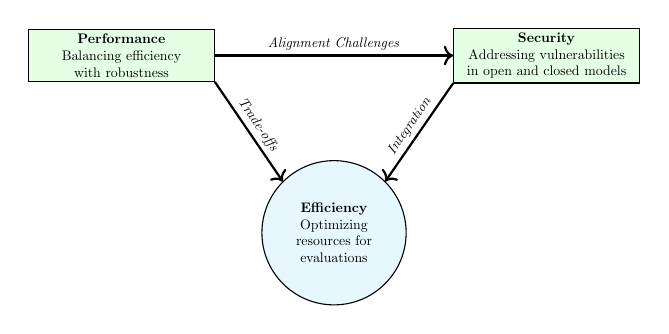
\begin{tikzpicture}[scale=0.9, every node/.style={scale=0.5}]
            % Nodes
            \node[draw, fill=green!10, text width=4.5cm, align=center] (perf) at (0, 0) {\textbf{Performance} \\ Balancing efficiency with robustness};
            \node[draw, fill=green!10, text width=4.5cm, align=center] (security) at (6, 0) {\textbf{Security} \\ Addressing vulnerabilities in open and closed models};
            \node[draw, circle,fill=cyan!10, text width=3cm,align=center] (efficiency) at (3, -2.5) {\textbf{Efficiency} \\ Optimizing resources for evaluations};

            % Connecting lines
            \draw[->, thick] (perf.south east) -- (efficiency.north west) node[midway, above, sloped] {\textit{Trade-offs}};
            \draw[->, thick] (security.south west) -- (efficiency.north east) node[midway, above, sloped] {\textit{Integration}};
            \draw[->, thick] (perf.east) -- (security.west) node[midway, above] {\textit{Alignment Challenges}};

            % % Main caption
            % \node[align=center, text width=11cm, below] at (3, -4) {
            %     \small These findings emphasize the need for balancing performance, security, and efficiency when evaluating LLMs. Joint consideration of these factors is crucial to developing safer, more reliable models.
            % };
        \end{tikzpicture}
        }
        \caption{Balancing performance, security, and efficiency.}
        \label{fig:tikz_perf_security_efficiency}
    \end{subfigure}%
    \hfill
    % Second TikZ Subfigure
    \begin{subfigure}[b]{0.48\textwidth} % Adjust the width as needed
        \centering
        \resizebox{\textwidth}{!}{%
        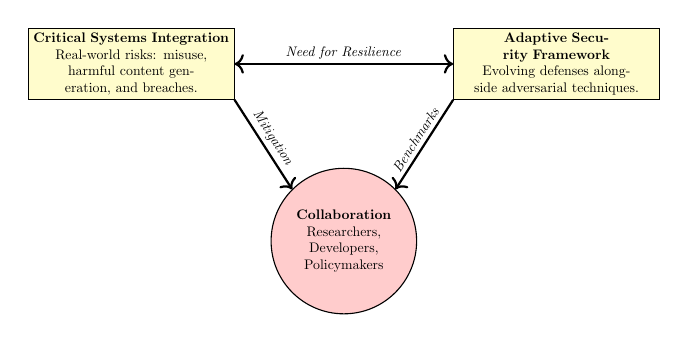
\begin{tikzpicture}[scale=0.9, every node/.style={scale=0.5}]
            % Critical Systems Integration
            \node[draw, rectangle, fill=yellow!20, text width=5cm, align=center] (integration) at (0, 0) {\textbf{Critical Systems Integration}\\ Real-world risks: misuse, harmful content generation, and breaches.};

            % Adaptive Security Framework
            \node[draw, rectangle, fill=yellow!20, text width=5cm, align=center] (framework) at (6, 0) {\textbf{Adaptive Security Framework}\\ Evolving defenses alongside adversarial techniques.};

            % Connection
            \draw[<->, thick] (integration.east) -- (framework.west) node[midway, above] {\textit{Need for Resilience}};

            % Collaboration Node
            \node[draw, circle, fill=red!20, text width=3cm, align=center] (collab) at (3, -2.5) {\textbf{Collaboration}\\ Researchers, Developers, Policymakers};

            % Arrows to Collaboration
            \draw[->, thick] (integration.south east) -- (collab.north west) node[midway, above, sloped] {\textit{Mitigation}};
            \draw[->, thick] (framework.south west) -- (collab.north east) node[midway, above, sloped] {\textit{Benchmarks}};
        \end{tikzpicture}
        }
        \caption{Integration of systems and collaboration.}
        \label{fig:tikz_critical_integration}
    \end{subfigure}

    % Main Caption
    \caption{A visual representation of key challenges and solutions in LLM security evaluation.}
    \label{fig:combined_tikz_figures}
\end{figure}

\noindent As LLMs integrate into critical systems, these vulnerabilities pose real-world risks such as misuse, harmful content generation, and security breaches. To address these challenges, adaptive security frameworks and collaborative efforts among researchers, developers, and policymakers are essential for establishing standardized benchmarks and ensuring safe deployment of LLMs.



\section{Conclusion}

\texttt{EasyJailbreak} represents a significant advancement in the field of securing Large Language Models (LLMs) against the evolving threat of jailbreak attacks. By introducing a unified and modular framework, it simplifies the evaluation and development of both attack and defense strategies, offering compatibility across a broad spectrum of LLMs.

\subsection*{Key Findings}
The evaluation conducted using \texttt{EasyJailbreak} reveals critical vulnerabilities within even the most advanced LLMs. With an alarming 60\% average breach probability across various jailbreak methods, the findings emphasize the pressing need for robust security measures. Notably:
\begin{itemize}
    \item Even advanced models like GPT-3.5-Turbo and GPT-4 exhibited average Attack Success Rates (ASR) of 57\% and 33\%, respectively.
    \item The framework's ability to uncover vulnerabilities highlights the importance of comprehensive and standardized testing methodologies in enhancing LLM security.
\end{itemize}

\subsection*{Future Directions}
\texttt{EasyJailbreak} equips researchers with essential tools to innovate and improve LLM security. The modular architecture not only facilitates the benchmarking of existing methods but also encourages the development of novel defenses against emerging threats. Potential areas for future exploration include:
\begin{itemize}
    \item Designing adaptive defense strategies tailored to evolving adversarial techniques.
    \item Expanding the framework's capabilities to include more sophisticated evaluators and attack recipes.
    \item Collaborating across the research community to establish standardized benchmarks for LLM security.
\end{itemize}

\subsection*{Ethics and Responsible Usage}
Given the dual-use potential of \texttt{EasyJailbreak}, the framework is intended strictly for ethical and constructive purposes. The authors advocate for responsible disclosure of vulnerabilities, ensuring developers have the opportunity to address flaws before public dissemination. The goal is to advance the security and reliability of LLMs while promoting collaboration across the cybersecurity ecosystem.
\\  \\
In conclusion, \texttt{EasyJailbreak} sets a new standard for LLM security evaluation and improvement. By equipping researchers with powerful tools and fostering innovation in defense strategies, it paves the way for safer and more resilient large language models.

% \bibliographystyle{plain}
% \bibliography{ref}
\printbibliography

\end{document}